\section{Introduction}
Getting robots to execute complex,
goal-directed tasks in unstructured settings remains a major challenge.

In particular, deformable object manipulation presents an interesting challenge.
These problems are characterized by state and action spaces that are high-dimensional 
and continuous and direct solutions require reasoning about dynamics of complex object 
through contact.
Determing a correct underlying representation of these objects is itself a difficult problem,
and often requires complicated task specific implementations.

A recent approach applies \emph{trajectory transfer} through the use of
non-rigid registration to deformable object manipulation, and thus avoids
direct manipulation of object representations~\cite{Schulmanetal_IROS2013, Schulmanetal_ISRR2013}.
Trajectory transfer fits a
function $f:\mathbb{R}^3 \rightarrow \mathbb{R}^3$ that warps a demonstration
scene to a novel setting.  The demonstrated trajectory is warped with this
function and the result is executed in the current scene.  This has been shown
to be effective for many complex tasks, including knot-tying and suturing.

For complex tasks, often demonstrations correspond to steps in the task, rather
than the entire task itself. Figure~\ref{fig:knot_steps} shows an example
for tying an overhand knot.
In general, a single demonstration for a step in the task cannot be expected
to cover all possible scenarios that arise during execution.
The natural solution to this is to use a library of demonstrations with
multiple demosntrations for each step.

However, realizing these benefits requires a robust technique to select a good trajectory to
transfer.
This is not an easy task.
Certain trajectories will generalize better than others, and particular sequences of 
demonstrations may perform tasks more efficiently than others.
The existence of poor or brittle demonstrations can very negatively 
effect performance.
For example, a demonstration in knot tying that involves a grasp
unnecessarily close to the edge of the rope may generalize poorly
to new scenes, compared to other more robust demonstrations of the task.

The original paper presenting this approach
prescribes choosing the trajectory segment from the demonstrations
library with the lowest warping cost onto the current scene~\cite{Schulmanetal_ISRR2013}.
This approach does not account for the inherent generalizability
of a particular demonstration. For brittle demonstrations (e.g. grabbing
near the edge of a rope), a small change in the rope can have low registration
cost but the transferred trajectory will fail.
As a result, such an approach may fail to accomplish tasks
that would be possible with a different sequence of trajectories.

\begin{figure}[t]
  \centering
    \noindent
    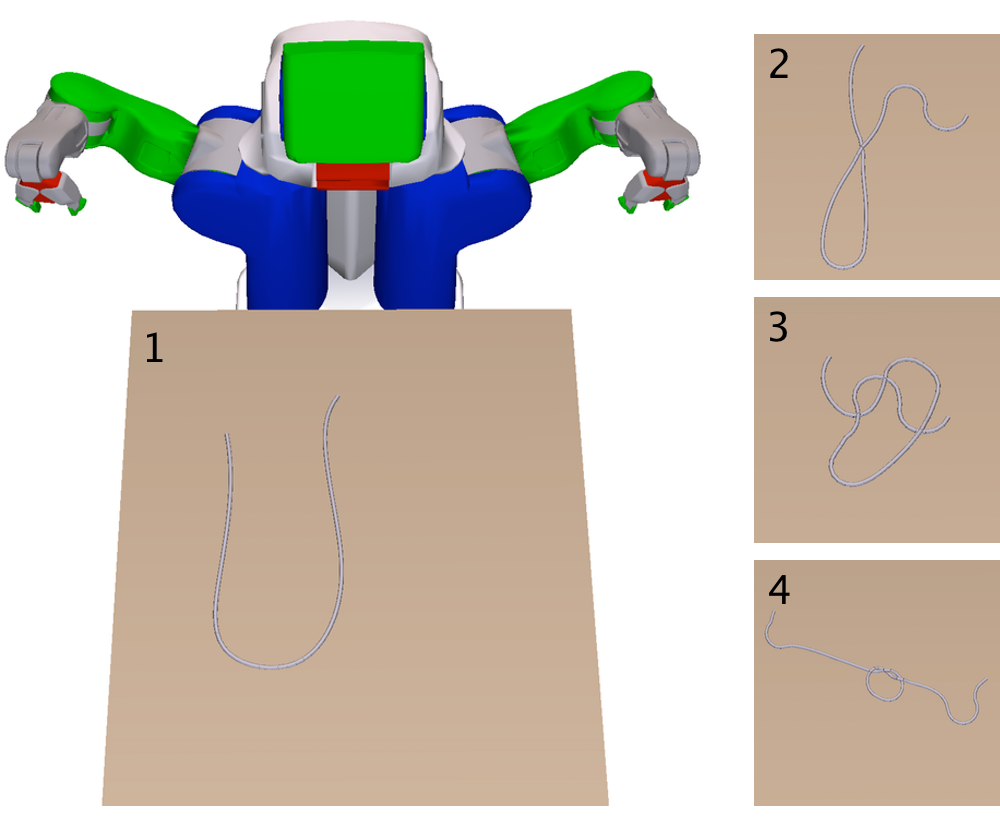
\includegraphics[width=0.45\textwidth]{figures/knot_steps_num.png}
  \caption{The overhand knot manipulation task in our benchmark.
           A standard knot tie takes three steps, as shown in this
           particular execution from our benchmark.}
  \label{fig:knot_steps}
\end{figure}

%TODO: make into list; link to sections/subsections in the paper
In this paper, we present a solution to the demonstration selection problem that
can account for the variability in robustness of demonstrations and the
sequential nature of our tasks. Our contributions are as follows:
(i) we formulate the demonstration selection problem as a Markov Decision
Process (MDP); (ii) we present Max-Margin Q-Learning (\mmql{}), a method for
approximating Q-functions from expert demonstrations that accounts for the
optimality of the expert's actions; (iii) we describe task-independent
features that are rich enough to allow learning but make no additional
assumptions beyond those of trajectory transfer; (iv) we develop an unsupervised
labeling method that we call Leave-One-Out Labeling (LOOL) that allows
us to apply \mmql{} with no human input beyond the initial demonstrations.

We validate our approach on an overhand knot-tying task. We contribute a
benchmark for this task (available at \href{https://sites.google.com/site/rss2014mmql}{sites.google.com/site/rss2014mmql}). The nearest
neighbor approach described in \citet{Schulmanetal_ISRR2013} achieves a
68.8\% success rate. The greedy policy with respect to our learned
approximate Q-function achieves a success rate of 85.6\%. Augmenting our
policy with a simulator and beam search raises the success rate to 95.2\%.
The best possible success rate with our demonstration library is 95.2\%.

While our running example and experiments deal with knot tying, our presented
\mmql{} approach is general and makes no assumptions about the task
beyond those of trajectory transfer.
